\chapter{ISP 与图像算法}
\oneline{ISP 层由像素处理链与两个统计-控制闭环组成:4:1 位宽变换 $\to$ DPC 坏点
修复 $\to$ 去马赛克 $\to$ 白平衡/数字增益的流式像素链,叠加 AWB 增益回注与
v38 自动曝光 PID——AE 经 I2C 调节传感器曝光,达到上限后调节 FPGA 数字增益,
模拟增益保持手动;再加七种实时风格化模式。本章给出原理、判据与验证。}

\section{ISP 流水与 3A 闭环}

ISP(Integrated Signal Processing)层完成"RAW10 像素组 $\to$ 校色后 RGB888 流"
的全部处理,并承载经典 3A 闭环中的两个——自动曝光(AE)与自动白平衡(AWB)。
整体结构如图~\ref{fig:isp3a} 所示:\textbf{像素处理链}为流式流水(4:1 位宽变换
gearbox $\to$ DPC $\to$ 去马赛克 $\to$ color\_correct,全部常数延迟);两个
\textbf{统计-控制闭环}的口径刻意分离——AWB 在\textbf{校正前}的 RGB 上估计
传感器原始色偏,AE 在\textbf{校正后}的图像上测亮度(与输出画面同口径)。
AWB 闭环把算出的绝对增益回注 color\_correct(下一帧生效);v38 AE 闭环把曝光码
经 I2C 请求/确认桥写入传感器,触及曝光上限后在像素域提高数字增益(1$\sim$4 倍);
模拟增益保持手动设定。网络手动命令可随时接管
任一闭环(见第 4 章)。

\begin{figure}[H]\centering
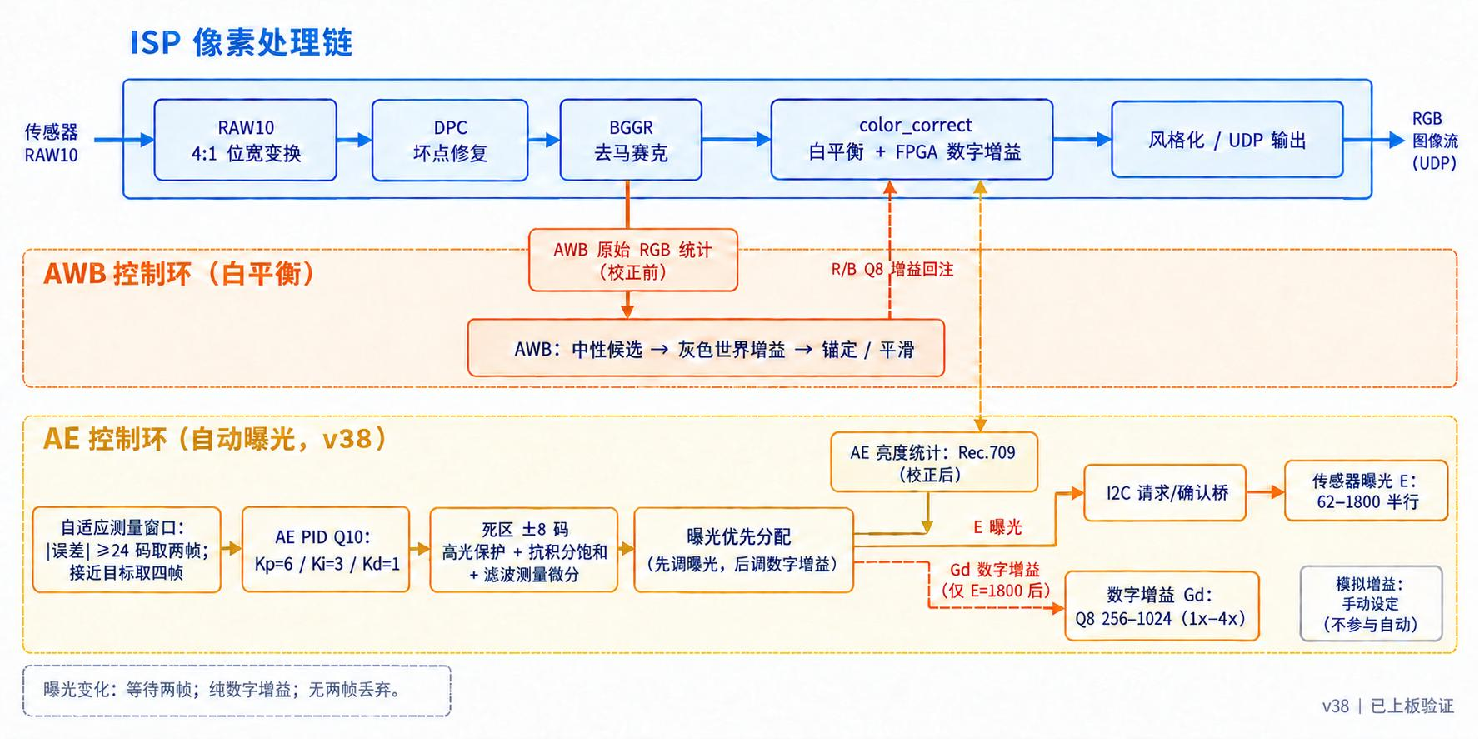
\includegraphics[width=\textwidth]{figs/fig_isp_3a.pdf}
\caption{ISP 层与 3A 闭环:像素处理链(实线)与 AE/AWB 统计-控制回路}
\label{fig:isp3a}
\end{figure}

\section{坏点检测与修复:RAW 域同色对角判据(DPC)}

坏点(sensor 出厂缺陷或高增益下的离群像素)若留到彩色重建之后才处理,一个坏点会经
双线性插值扩散成 5 像素的十字彩色斑;因此 DPC 插在位宽变换之后、去马赛克之前的
RAW10 域,此时一个坏点只是一个孤立的 10\,bit 值,处理代价最小。

\textbf{判据:}Bayer 排列下,$3\times3$ 窗口内与中心同色的恰是 4 个对角点
($d_1=p_{00}$、$d_2=p_{02}$、$d_3=p_{20}$、$d_4=p_{22}$)——这对任何 CFA 相位都
成立,无需相位信息。坏点的本质是"与所有同色邻居同时、同向、不连续地偏离",据此
两级判据:
\begin{align*}
\text{亮点坏点:}\quad & c>\max_i d_i+\mathrm{TH}\quad\text{且}\quad c>\overline{d}+\mathrm{TH}_2;\\
\text{暗点坏点:}\quad & c+\mathrm{TH}<\min_i d_i\quad\text{且}\quad c+\mathrm{TH}_2<\overline{d},
\end{align*}
其中 $\overline{d}=\frac{1}{4}\sum_i d_i$。只看 max/min 单阈值会把噪声尖峰误判成
坏点(高增益时尤甚),与均值的偏离量能滤掉大部分噪声;而"四个邻居全部同向偏离"
本身也抗纹理误检——细线、边缘上邻居一亮一暗、方向不一致,不会触发。

\textbf{矫正:}命中才把中心替换为 4 个同色邻居的中位数,其余像素原样直通——与全局
中值滤波的本质区别是只动被判定的像素,不伤分辨率。中位数与 max/min 共用同一级
sort4 部分网络(5 个比较器)。判据与矫正采用两级流水:第 1 拍寄存 sort4 输出与
4 邻居均值,第 2 拍只做阈值加法、比较与矫正选择,满足 100\,MHz 时序;整级固定
4 拍。两处边界选择"不矫正"(宁漏勿错):复制边界处邻居与中心等值时判据自然失效;
每行第 1 个输出槽位的中心落在第 0 列,其"水平邻居"是上一行行尾回绕像素,用列
计数识别并直接旁路。

\textbf{验证:}单元自检注入坏点全部按邻居中位数修复、平滑背景零误检、随机纹理下
与 golden 参考模型逐位一致;全量联合仿真注入亮暗坏点 24 个,24/24 修复、邻域残差
全 0,坏点趟 vs 干净趟全帧 PSNR 101.09\,dB。放大图直观显示:单像素 RAW 坏点经
插值会变成彩色伪影,DPC 修好后输出与干净趟完全一致——坏点必须在 RAW 域、去马赛克
之前修的实证。

\section{去马赛克:BGGR 双线性彩色重建}

Bayer 原始数据的每个像素只携带单一颜色分量,必须插值出全彩;插值相位必须与传感器
的 Bayer 排列严格一致。记 $3\times3$ 窗口及其中心像素为
\begin{equation*}
W=\begin{pmatrix}p_{00}&p_{01}&p_{02}\\ p_{10}&p_{11}&p_{12}\\ p_{20}&p_{21}&p_{22}\end{pmatrix}
\qquad\text{中心像素 }p_{11},
\end{equation*}
插值输出记 $(\hat R,\hat G,\hat B)$,则四种相位为
\begin{align*}
B\text{ 中心:}\quad & \hat B=p_{11},\quad \hat G=\tfrac{1}{4}\bigl(p_{01}+p_{21}+p_{10}+p_{12}\bigr),\quad \hat R=\tfrac{1}{4}\bigl(p_{00}+p_{02}+p_{20}+p_{22}\bigr);\\
R\text{ 中心:}\quad & \hat R=p_{11},\quad \hat G=\tfrac{1}{4}\bigl(p_{01}+p_{21}+p_{10}+p_{12}\bigr),\quad \hat B=\tfrac{1}{4}\bigl(p_{00}+p_{02}+p_{20}+p_{22}\bigr);\\
G\text{ 中心(偶行):}\quad & \hat G=p_{11},\quad \hat R=\tfrac{1}{2}\bigl(p_{01}+p_{21}\bigr),\quad \hat B=\tfrac{1}{2}\bigl(p_{10}+p_{12}\bigr);\\
G\text{ 中心(奇行):}\quad & \hat G=p_{11},\quad \hat B=\tfrac{1}{2}\bigl(p_{01}+p_{21}\bigr),\quad \hat R=\tfrac{1}{2}\bigl(p_{10}+p_{12}\bigr).
\end{align*}
即已知色取自身,缺失色分别用同色正邻域均值或对角均值插值;输出 8\,bit 取 10\,bit
结果的高 8 位。固定 3 拍延迟、复制边界(首行首列同样正确)。一处关键标定:数据到达
时行相位比 BGGR 排列假设差一整行,因此行偶判定使用行计数低位本身——该相位以色块
自检(灰底放置红/绿/蓝/白块,逐行核对输出颜色)确认;行列计数与帧起始的对齐保证
色平面不错位。

\section{色彩校正与自动白平衡(AWB)}

color\_correct 在去马赛克之后完成白平衡,每像素校正为
\begin{equation*}
O_c=\min\bigl(255,\ \mathrm{round}(I_c\,g_c/256)\bigr),\qquad c\in\{R,B\},\quad g_G\equiv 256,
\end{equation*}
即 Q8 定点乘法(8$\times$9\,bit 取高位、四舍五入、饱和到 255),$G$ 通道锚定
1.0$\times$——Von Kries 形式只调色温不漂移亮度;另支持全模式 R/B 通道互换
(色序错配一键修)。白平衡有四种工作模式:\textbf{标定预设}(出厂标定增益,
R344/G256/B451)、\textbf{色温 K 值}(拖动色温 2500$\sim$10000\,K,经光源近似
曲线换算 R/B 增益,6500K 为参考锚点)、\textbf{手动 RGB}(Q8 增益
64$\sim$1024,256 = 1.0$\times$)与\textbf{自动场景(AWB 闭环)}。

\textbf{AWB 闭环}是 ISP 的统计-控制回路,统计在\textbf{未校正}的 RGB(去马赛克
输出、数字增益之前)上进行——估计的是传感器原始色偏,不受当前增益影响;闭环
每帧执行四步:

\textbf{(1) 中性候选判据。}先把三通道按标定先验加权
\begin{equation*}
R'=\tfrac{344}{256}\,R,\qquad G'=G,\qquad B'=\tfrac{451}{256}\,B,
\end{equation*}
在先验拉平后的色度上判中性。宽松判据为
\begin{equation*}
2\bigl(\max_c C'_p-\min_c C'_p\bigr)\le\max_c C'_p,\qquad
32<Y_p<230,\qquad 2<I_{c,p}<250,
\end{equation*}
即色度散布不超过最大通道的一半、亮度与各通道都在非黑非削顶的窗内。保守判据
(现行配置)收紧为 $8(\max-\min)\le\max$(散布 $\le$ 1/8)外加亮度窗
$64\le G\le224$、$\max<235$、$\min>32$,并要求\textbf{四象限多样性}:画面四等分,
每象限中性样本 $\ge WH/2000$,至少 2 个象限有效才接受本帧估计(防单一物体
主导统计);象限 $\ge$3 且 $n\ge 5\%\,WH$ 判为强置信。

\textbf{(2) 接受条件与冻结守卫。}全帧统计完整(样本数 $=WH$)、中性样本数
$n\ge\max(WH/100,16)$、$\sum_{\mathcal N}R$ 与 $\sum_{\mathcal N}B$ 非零且象限
足够;任一不满足即\textbf{冻结}当前增益并上报原因码(暗场/过曝/样本不足/
象限不足)——宁可不校,不可误校。

\textbf{(3) 增益生成。}对中性样本集 $\mathcal N$ 以 $G$ 为基准求灰色世界增益,
帧尾以 Q8 定点除法完成:
\begin{equation*}
g_R^{\mathrm{cand}}=\mathrm{clip}_{[128,\,1024]}\Bigl(\frac{\sum_{p\in\mathcal N}G_p}{\sum_{p\in\mathcal N}R_p}\Bigr),\qquad
g_B^{\mathrm{cand}}=\mathrm{clip}_{[128,\,1024]}\Bigl(\frac{\sum_{p\in\mathcal N}G_p}{\sum_{p\in\mathcal N}B_p}\Bigr),
\end{equation*}
自动模式限幅 $0.5\times\sim4\times$。

\textbf{(4) 先验锚定与时域平滑。}保守模式下候选先夹到标定基准
$g_{\mathrm{base}}$(R344/B451)的 $\pm25\%$ 邻域再与之混合,随后与当前增益做
一阶惯性平滑:
\begin{align*}
\text{锚定:}\quad & \hat g=\mathrm{clip}\bigl(g^{\mathrm{cand}},\
[\tfrac34 g_{\mathrm{base}},\ \tfrac54 g_{\mathrm{base}}]\bigr),\qquad
g^{\mathrm{mix}}=\begin{cases}\tfrac12\bigl(g_{\mathrm{base}}+\hat g\bigr), & \text{强置信}\\[2pt]
\tfrac14\bigl(3g_{\mathrm{base}}+\hat g\bigr), & \text{弱置信}\end{cases};\\[4pt]
\text{平滑:}\quad & g^{(t)}=\begin{cases}
\bigl(3g^{(t-1)}+g^{\mathrm{mix}}+2\bigr)\gg 2, & \text{宽松模式}\\[2pt]
\bigl(15g^{(t-1)}+g^{\mathrm{mix}}+8\bigr)\gg 4, & \text{保守模式}\end{cases}
\qquad(g_R,g_B\ \text{各自独立}) .
\end{align*}
两级设计让单帧统计噪声只占 1/4(宽松)乃至 1/16(保守)的权重:静态场景增益
快速锁死不振荡,真实色偏仍稳定收敛;实测固定场景自动增益收敛于标定值
(R344/G256/B451)。自动模式不显示伪造的"测得色温"。模式切换与增益设置均经
网络命令运行时生效(见第 4 章),预览与保存图均为正确 RGB 顺序。

\section{自动曝光(AE):固定点 PID 与曝光优先分配}

当前 v38 版本的 AE 采用帧事件驱动的固定点 PID。控制器测量白平衡校正后的 RGB
亮度(与输出图像口径一致),每帧统计亮度均值和高亮像素数;空统计帧不参与控制。
目标默认值为 112,以实际状态包回报的目标为准。高亮像素比例超过 5\% 时启用
高光保护:目标可按当前均值下调并保持,避免控制器在高反差场景中一边压高光、一边
试图抬升全帧均值。高光条件解除且亮度明显偏离时,目标恢复默认值。

测量采用自适应窗口:误差绝对值达到 24 个亮度码时使用最近两帧平均,接近目标时
累计四帧平均。目标死区为 $\pm8$ 码。误差、积分和测量微分均在 Q2 亮度单位中
计算;误差反向时清除积分与微分历史。积分限幅为 $[-512,512]$,对控制输出限幅并
使用抗积分饱和。默认 PID 系数为 Q10 编码 $K_p=6$、$K_i=3$、$K_d=1$,实际
乘数分别为 $6/1024$、$3/1024$、$1/1024$。微分项采用测量微分并作一阶平均:
\begin{equation*}
D_{raw}=\bar Y_{t-1}-\bar Y_t,\qquad
D_t=\frac{D_{t-1}+D_{raw}}{2},\qquad
C=\operatorname{clip}_{\pm C_{max}}\left(\frac{K_pe+K_iI+K_dD_t}{4\cdot1024}\right),
\end{equation*}
其中误差达到 24 码时 $C_{max}=256$,接近目标时为 64;微分项可以抑制
或暂缓调整,但不能使执行方向与当前误差相反。实际硬件内部保留 Q2 精度并按流水
阶段完成运算。

控制器调节总曝光量 $U=E\,G_d$,其中 $E$ 为传感器曝光半行码、$G_d$ 为 Q8
FPGA 数字增益。每次更新按 PID 输出比例改变 $U$,最小变化量为 $1\times256$
(Q8 单位),随后按如下优先级分配:
\begin{align*}
E&\in[62,1800],\qquad G_d\in[256,1024]\quad(1\times\sim4\times);\\
U\le1800\times256&\Rightarrow G_d=256,\quad E\approx U/256;\\
U>1800\times256&\Rightarrow E=1800,\quad G_d\approx U/1800.
\end{align*}
因此先用曝光,触及安全上限后才增加 FPGA 数字增益;模拟增益保持用户手动设定。
曝光上限仍由传感器接近满帧时的读出窗偏移限制,原因见第 2 章。亮度变暗时
数字增益放大噪声,故暗场质量仍需实机评估。

执行采用请求/确认互斥。曝光写入成功后保留两帧稳定保护;纯 FPGA 数字增益在
SOF 锁存,确认帧已经是新增益图像,因此不再丢弃两帧。手动事务会清空旧 PID
历史。6/3/1 闭环模型在亮场和暗转亮场比冻结的 4/1/0 控制器更快,暗场相同、
极暗场略慢;稳定窗口与交替亮度检查无反复调节,460 帧完整视频 RTL 链路模型
通过。上述为仿真对比结论;v38 源码已上板验证,具体板级 AE 响应以对应实测记录为准,
不将仿真差异当作板测指标。
\section{七模式风格化算法}

风格化级以公共像素流接口挂在白平衡之后、推流之前,提供七种实时模式,板上由两个
功能键切换(下一模式/上一模式,切换在帧首生效,状态文字与画面同帧):

\begin{table}[h!]\centering\small
\caption{七种风格化模式}
\begin{tabular}{clp{9.8cm}}
\toprule
模式 & 名称 & 实现 \\
\midrule
0 & 原图 & 白平衡结果直通 \\
1 & 灰度 & $Y=(R+2G+B)\gg2$ 三通道同值 \\
2 & 二值化 & 亮度与阈值比较 \\
3 & Sobel 边缘 & 亮度梯度 $|G_x|+|G_y|$,独立高低阈值双门限 + 滞后连接;
低阈值默认联动为高阈值一半,可解除;两模式参数各自记忆,复位恢复默认 \\
4 & 卡通 & 中值滤波(保边平滑)$\to$ 每通道 3 位颜色量化 $\to$ 黑描边 \\
5 & 素描 & 白底黑线,与边缘共用判决,独立阈值与线宽(加粗) \\
6 & 复古暖色 & 定点 sepia 矩阵变换 \\
\bottomrule
\end{tabular}
\end{table}

边缘与素描的高低阈值、线宽经 GUI 实时可调(如边缘推荐低 45/高 90,素描低 50/
高 100;主阈值越低细节越多);模式切换经帧首生效保证无撕裂。全部模式与 Python
位级参考对拍,并参加七模式轮换长时间运行验证(平均 29.965\,fps、完整率 100\%)。
